% Capítulo 5 — Avaliação (orçamento: ~16 pp)
% Uma secção por QI. Cada uma: pergunta, como se mediu, resultado, e o que NÃO se pode concluir.
% ️ Usar o chão CORRIGIDO da precisão@orçamento (aleatório 0.379), nunca o 0.163 alfabético.

\chapter{Avaliação}
\label{cap:avaliacao}

\section{Como está montado este capítulo}
\label{sec:av_montagem}

Cada uma das três perguntas de investigação tem aqui a sua secção. Todas seguem a mesma forma, de
propósito:

\begin{enumerate}
  \item a pergunta;
  \item como foi medida, e contra que alternativa;
  \item o resultado;
  \item \textbf{o que este resultado não permite concluir}.
\end{enumerate}

O quarto ponto é o que separa uma avaliação de uma demonstração. Todos os números deste capítulo são
produzidos por procedimentos automáticos com semente fixa: correr outra vez sobre os mesmos dados dá
exatamente os mesmos valores.

Falta explicar uma assimetria, antes que ela pareça um esquecimento. O
Capítulo~\ref{cap:metodologia} descreve \emph{quatro} técnicas e este capítulo tem \emph{três}
perguntas de investigação. A técnica que fica de fora é a decomposição de um movimento, e a razão
por que fica é metodológica e não de conveniência: não existe resposta certa contra a qual a
comparar. A Secção~\ref{sec:av_decomposicao} trata-a à parte e explica o que, nela, ainda assim se
pode medir.

\section{Como se lê cada número deste capítulo}
\label{sec:av_metricas}

Um resultado vale o que vale a medida que o produziu, e este capítulo usa cinco. Esta secção define
cada uma e, sobretudo, fixa o seu \textbf{chão} --- o valor que um método sem informação nenhuma
obtém --- porque uma medida lida sem o seu chão dá a conclusão errada, e este capítulo documenta
três ocasiões em que isso aconteceu.

Todas assentam nas quatro combinações entre o que o sistema afirma e o que a realidade tem:
verdadeiros e falsos positivos, verdadeiros e falsos negativos. Os dois erros não são simétricos e
custam coisas diferentes: um falso positivo gasta a atenção de quem lê, um falso negativo deixa
passar o dia que interessava.

A \textbf{precisão} é a fração de acertos entre as vezes em que o sistema falou,
$\mathrm{VP}/(\mathrm{VP}+\mathrm{FP})$; a \textbf{cobertura} é a fração dos casos relevantes que
ele apanhou, $\mathrm{VP}/(\mathrm{VP}+\mathrm{FN})$. Uma sobe à custa da outra, e uma regra que
fale quase sempre atinge cobertura alta com precisão baixa.

\subsection{O \texorpdfstring{$F_1$}{F1}}
\label{sec:av_f1}

O $F_1$ é a média harmónica das duas, $2 \cdot \frac{P \cdot C}{P + C}$, e puxa o resultado para o
pior dos dois valores, o que impede que um extremo seja premiado. Para o \emph{z}-score, com
precisão $0.381$ e cobertura $0.800$, dá $0.516$; para a regra fixa, com precisão $0.122$ e
cobertura $0.992$, dá $0.218$.

\subsection{A precisão@\texorpdfstring{$k$}{k}}

A recuperação de precedentes devolve uma lista ordenada, e o utilizador lê apenas as primeiras.
Avalia-se com uma medida sensível à ordem \autocite{manning2008ir}: a fração dos $k$ primeiros
resultados que são relevantes, com $k = 5$, que é o que cabe num alerta. O seu chão não é zero: uma
escolha ao acaso entre cinco setores de tamanhos diferentes acerta $0.240$ das vezes.

\subsection{A PR-AUC}
\label{sec:av_prauc}

O modelo de triagem devolve uma probabilidade, não uma decisão. Cada limiar possível dá um par
(cobertura, precisão), e o conjunto desses pares desenha a curva de precisão--cobertura; a
\gls{PRAUC} é a área debaixo dela, e resume o modelo em todos os limiares de uma vez em vez de o
julgar num limiar escolhido à mão.

O seu chão é a proporção de casos positivos nos dados: um modelo que atribua a mesma probabilidade
a tudo obtém exatamente essa proporção. No bloco de teste ela é $0.378$, e é contra esse valor, e
não contra zero, que todas as PR-AUC deste capítulo devem ser lidas. Prefere-se à percentagem de
acertos porque, com classes desequilibradas, responder sempre ``não é importante'' acerta $62.2\%$
das vezes sem ter aprendido nada.

\subsection{O Brier}
\label{sec:av_brier}

As medidas anteriores olham para a \emph{ordenação}. O Brier olha para o \emph{valor} da
probabilidade, que é o que o sistema mostra ao utilizador: é a média do quadrado do erro entre a
probabilidade anunciada e o que aconteceu, e aqui quanto menor melhor. O quadrado penaliza mais do
que proporcionalmente os enganos confiantes, que é a propriedade desejada num sistema que exibe
percentagens a quem não as sabe questionar. O seu chão fecha a conta: um modelo que anuncie $1$
para tudo paga a fração de casos não importantes, $1 - 0.378 = 0.622$, que é exatamente o valor
reportado para esse modelo na Tabela~\ref{tab:av_triagem}.

\begin{table}[ht]
\caption[As medidas usadas e o que cada uma responde]{Cada medida, a pergunta a que responde, o seu
chão de referência, e onde aparece neste capítulo.}
\label{tab:av_metricas}
\centering
\small
\begin{tabular}{L{0.15\textwidth} L{0.34\textwidth} L{0.20\textwidth} C{0.13\textwidth}}
\toprule
\tabhead{Medida} & \tabhead{Responde a} & \tabhead{Chão} & \tabhead{Usada em} \\
\midrule
Amplitude de disparo & O detetor comporta-se do mesmo modo em empresas diferentes? & zero seria o
ideal & \gls{QI}1 \\
\addlinespace
$F_1$ & Acerta quando fala, e fala quando devia? & depende dos dados & \gls{QI}1 \\
\addlinespace
Precisão@5 & Das cinco que mostro, quantas são relevantes? & $0.240$ (acaso medido) & \gls{QI}2 \\
\addlinespace
PR-AUC & Ordena bem, seja qual for o limiar? & $0.378$ (a prevalência) & \gls{QI}3 \\
\addlinespace
Brier & A percentagem anunciada é honesta? & $0.622$ (alertar sempre) & \gls{QI}3 \\
\bottomrule
\end{tabular}
\end{table}

A primeira linha da Tabela~\ref{tab:av_metricas} é a única medida deste capítulo que não usa
rótulos: a amplitude de disparo mede a diferença entre a empresa em que o detetor mais fala e
aquela em que menos fala, e parte apenas do princípio de que um bom detetor universal se deve
comportar de forma parecida em empresas diferentes.

\section{QI1: detetar o que é invulgar}
\label{sec:av_qi1}

\emph{Um \emph{z}-score deslizante deteta movimentos invulgares de forma mais consistente do que uma
regra fixa?} \textbf{Sim, e com uma margem grande.}

\subsection{Como foi medido}

Foram usados três anos de cotações diárias de quinze empresas grandes, entre junho de 2023 e junho de
2026, ou seja, cerca de 750 dias por empresa.

São quinze, e não as doze que o sistema vigia em produção. A diferença é de propósito: a avaliação
quer \emph{variedade} de volatilidade, para o argumento da consistência ter sobre o que incidir; a
lista de produção é uma escolha de produto e não uma amostra. Confundir as duas seria avaliar o
detetor exatamente no conjunto que ele foi montado para servir.

O argumento principal não precisa de rótulos nenhuns, e é por isso que é o principal. Um bom detetor
universal deve disparar a um ritmo \textbf{parecido} em empresas diferentes. Se dispara muito numa e
quase nada noutra, o que está a medir é a volatilidade da empresa e não a raridade do dia.

Como argumento de apoio, usou-se também um rótulo aproximado: considera-se ``dia extremo'' um dia no
percentil 99 dos retornos \emph{daquela} empresa. É um rótulo imperfeito, porque é ele próprio
relativo à volatilidade, e por isso vem em segundo lugar.

\subsection{Resultado}

A Tabela~\ref{tab:av_disparo} mostra o argumento principal.

\begin{table}[ht]
\caption[Consistência da taxa de disparo]{Com que frequência cada método dispara, entre as quinze
empresas. O que interessa é a \textbf{amplitude}: quanto menor, mais consistente é o detetor.}
\label{tab:av_disparo}
\centering
\begin{tabular}{l c c c}
\toprule
\tabhead{Método} & \tabhead{Taxa mínima} & \tabhead{Taxa máxima} & \tabhead{Amplitude} \\
\midrule
\emph{z}-score (janela 20) & $0.016$ & $0.031$ & $\mathbf{0.015}$ \\
Limiar fixo ($|r| \ge 3\%$) & $0.009$ & $0.353$ & $0.344$ \\
\bottomrule
\end{tabular}
\end{table}

A Figura~\ref{fig:av_disparo} mostra a mesma informação empresa a empresa.

A diferença é de mais de vinte vezes. O limiar fixo dispara em $0.9\%$ dos dias na empresa mais calma
e em $35.3\%$ dos dias na mais volátil, ou seja para uma delas quase nunca diz nada e para a outra
fala um dia em cada três, ao passo que o \emph{z}-score se mantém entre $1.6\%$ e $3.1\%$ em todas
elas.

\begin{figure}[ht]
\centering

\includegraphics[width=0.92\textwidth]{figures/eval_anomaly_firing_rate.pdf}
\caption[Taxa de disparo por empresa]{A mesma informação, empresa a empresa. As barras do limiar
fixo acompanham a volatilidade de cada ação; as do \emph{z}-score mantêm-se quase constantes.}
\label{fig:av_disparo}
\end{figure}

Contra o rótulo aproximado, o \emph{z}-score obtém $F_1 = 0.516$ contra $0.218$ do limiar fixo.

\paragraph{E é preciso dizer o que a amplitude sozinha não exclui, porque sozinha não exclui muito.}
A medida principal desta secção não tem chão em zero: tem o zero como ótimo, e o ótimo é atingível
por um método que não sabe nada. Um detetor que assinalasse, em cada empresa, uma fração fixa de
dias \emph{escolhidos ao acaso} teria amplitude praticamente nula, ou seja bateria o \emph{z}-score
exatamente na medida que aqui se elege como principal. Não precisa de ser corrido para se saber:
é uma consequência da construção.

Isso não invalida a medida; obriga a lê-la com a outra ao lado, e é essa a razão de existirem duas.
A amplitude exclui o limiar fixo, que dispara conforme a volatilidade da empresa em vez da raridade
do dia. O $F_1$ exclui o disparo aleatório, que fica ao nível do acaso contra qualquer rótulo.
\textbf{Nenhuma das duas basta sozinha, e apenas a regra deslizante passa nas duas}, e é isso que
a Figura~\ref{fig:av_duasmedidas} desenha. Fica assim
escrito porque a formulação anterior --- ``o argumento principal não precisa de rótulos, e é por
isso que é o principal'' --- é verdadeira quanto à independência de rótulos e insuficiente quanto
ao que a medida prova.

\begin{figure}[!htbp]
\centering
\begin{tikzpicture}[x=1.05cm, y=0.95cm, font=\small]
  % eixos
  \draw[->, thick] (0,0) -- (8.4,0) node[below left=2pt and 0pt]{amplitude de disparo \emph{(menor é melhor)}};
  \draw[->, thick] (0,0) -- (0,5.2) node[above left=0pt and -12pt, rotate=90, anchor=south]{};
  \node[rotate=90, anchor=south] at (-0.7,2.6) {$F_1$ \emph{(maior é melhor)}};
  % regioes excluidas
  \fill[orange!10] (5.0,0) rectangle (8.4,5.2);
  \fill[orange!10] (0,0) rectangle (8.4,1.6);
  \draw[dashed, orange!70!black] (5.0,0) -- (5.0,5.2);
  \draw[dashed, orange!70!black] (0,1.6) -- (8.4,1.6);
  \node[orange!60!black, align=center, font=\scriptsize] at (6.7,4.4)
    {excluído pela\\amplitude};
  \node[orange!60!black, align=center, font=\scriptsize] at (3.0,0.3)
    {excluído pelo $F_1$};
  % pontos
  \fill[black] (0.6,3.9) circle (2.4pt);
  \node[right=3pt, align=left] at (0.6,3.9) {\textbf{\emph{z}-score}\\[-2pt]{\scriptsize $0.015$ · $0.516$}};
  \fill[gray!70] (0.5,0.8) circle (2.4pt);
  \node[right=3pt, align=left] at (0.5,0.9) {disparo aleatório\\[-2pt]{\scriptsize $\approx 0$ · acaso}};
  \fill[gray!70] (7.4,0.55) circle (2.4pt);
  \node[above=3pt, align=center] at (7.0,0.6) {limiar fixo\\[-2pt]{\scriptsize $0.344$ · $0.218$}};
\end{tikzpicture}
\caption[O que cada medida da QI1 exclui]{As duas medidas desta secção, e o que cada uma
consegue excluir sozinha. A amplitude exclui o limiar fixo, que dispara conforme a volatilidade
da empresa; o $F_1$ exclui o disparo aleatório, que atinge o ótimo da amplitude sem saber nada.
\textbf{Só a regra deslizante fica fora das duas zonas.} A posição do disparo aleatório é uma
consequência da construção e não uma medição, e está desenhada a cinzento por isso.}
\label{fig:av_duasmedidas}
\end{figure}

Uma ressalva sobre esta comparação: a janela do \emph{z}-score é variada mais abaixo, e o limiar
de $3\%$ da regra fixa \textbf{não é}. É o valor convencional e não foi otimizado. Um limiar mais
alto subir-lhe-ia a precisão à custa da cobertura, e não é evidente em que ponto o $F_1$ ficaria;
o que a comparação mostra com segurança não é que nenhum limiar fixo consegue melhor, é que um
limiar fixo mede a coisa errada, porque a mesma percentagem significa coisas diferentes em
empresas diferentes. Esse argumento não depende do valor escolhido.

\paragraph{Uma assimetria no padrão de evidência.}
Os números desta pergunta e da seguinte são pontos, sem intervalo. Os da
Secção~\ref{sec:av_qi3}, que é onde está o resultado que me contraria, levam reamostragem por
grupos e intervalos de confiança. É uma assimetria: os resultados que me favorecem estão a ser
julgados por um padrão mais fraco do que o que me desfavorece. A justificação parcial é que as
diferenças aqui são de outra ordem de grandeza --- $0.516$ contra $0.218$, ou uma amplitude de
$0.015$ contra $0.344$, não são $0.005$ --- e por isso nenhuma reamostragem plausível as
inverteria. Mas a justificação não é completa, porque dias da mesma empresa também não são
independentes aqui, e pela razão que este mesmo capítulo invoca a propósito do desvio ponderado:
os movimentos grandes andam em grupo. A comparação de recuperação, essa, passou a mostrar o
desvio sobre as cinco repetições, que já existia e não estava impresso.

\subsection{E contra métodos aprendidos?}

Faltava a comparação mais exigente: e se em vez de uma regra estatística se usasse um método de
aprendizagem automática desenhado para detetar anomalias?

Foram testados dois, sobre exatamente a mesma informação e com o mesmo cuidado de não usar o futuro:
\emph{Isolation Forest} \autocite{liu2008isolation} e \emph{Local Outlier Factor}
\autocite{breunig2000lof}. O resultado está na Tabela~\ref{tab:av_detetores}.

\begin{table}[ht]
\caption[A regra transparente contra dois métodos aprendidos]{Os três detetores, sobre os mesmos
dados e sob o mesmo protocolo.}
\label{tab:av_detetores}
\centering
\begin{tabular}{l c c c c}
\toprule
\tabhead{Detetor} & \tabhead{Precisão} & \tabhead{Cobertura} & \tabhead{$F_1$} & \tabhead{Amplitude} \\
\midrule
\emph{z}-score (a regra) & $0.407$ & $0.761$ & $\mathbf{0.530}$ & $\mathbf{0.017}$ \\
Isolation Forest & $0.158$ & $0.913$ & $0.269$ & $0.140$ \\
Local Outlier Factor & $0.163$ & $0.989$ & $0.280$ & $0.183$ \\
\bottomrule
\end{tabular}
\end{table}

\textbf{A regra transparente ganha aos dois.} Não por pouco: quase o dobro do $F_1$, e com uma
consistência entre empresas muito melhor. Os dois métodos aprendidos assinalam quase tudo
(cobertura altíssima) e acertam pouco (precisão baixa).

Uma nota para quem comparar esta tabela com a conta feita na Secção~\ref{sec:av_f1}, onde o mesmo
\emph{z}-score aparece com $F_1 = 0.516$. Os dois valores são reais e medem o mesmo detetor sob
protocolos diferentes: o $0.516$ é sobre todos os dias avaliados, ao passo que o $0.530$ desta tabela
é sobre a região que os \textbf{três} detetores conseguem pontuar, que é a única em que a comparação
entre eles é justa. Comparar cada método fora da região comum daria vantagem a quem pontua mais
dias. A amplitude segue a mesma regra e é por isso que aparece aqui como $0.017$ e na
Tabela~\ref{tab:av_disparo} como $0.015$: é o mesmo detetor, medido sobre menos dias.

Este é o primeiro de três casos, neste capítulo, em que uma técnica mais sofisticada foi comparada
de forma justa com uma mais simples e perdeu. É um resultado que vale por si: justifica por medição
a escolha do método simples, em vez de a justificar por preferência.

Interessa perceber \emph{porquê}, porque a explicação não é que os métodos sejam maus. Ambos
decidem o que é invulgar pela geometria dos dados, ainda que por vias opostas: o \emph{Isolation
Forest} recusa modelar o normal e isola diretamente o ponto raro, pela facilidade com que ele se
separa por cortes aleatórios \autocite{liu2008isolation}, enquanto o \emph{Local Outlier Factor}
compara a densidade em torno de cada ponto com a dos seus vizinhos \autocite{breunig2000lof}. São ambos
métodos não paramétricos, distintos da família \emph{estatística} que \textcite{chandola2009anomaly}
define como aquela que modela a distribuição dos dados normais, e foram construídos para dados com
muitas variáveis a interagir. Aqui não é esse o caso: há uma série
de retornos por empresa, cuja estrutura relevante é \emph{temporal}. O agrupamento de volatilidade, que os modelos \gls{ARCH} e \gls{GARCH} formalizam
\autocite{engle1982arch, bollerslev1986garch}, faz com que o que conta como invulgar mude ao longo
do tempo, e uma janela deslizante acompanha isso por
construção, enquanto um detetor ajustado ao conjunto todo tem de o inferir. O padrão de resultados
confirma-o: os dois métodos aprendidos assinalam demasiado, que é o que sucede quando se aplica uma
noção global de raridade a séries cuja escala varia.

A Figura~\ref{fig:av_detetores} mostra esta comparação em gráfico, e ao lado uma segunda que ainda
não foi discutida.

\begin{figure}[ht]
\centering

\includegraphics[width=0.88\textwidth]{figures/eval_anomaly_detectors.pdf}
\caption[A regra contra os métodos aprendidos]{À esquerda, os três detetores sobre a mesma região
pontuada e com o mesmo cuidado de não usar o futuro. À direita, uma segunda comparação, entre duas
maneiras de estimar a volatilidade: a que o sistema usa e uma alternativa. Está discutida a seguir,
porque o resultado não foi o esperado.}
\label{fig:av_detetores}
\end{figure}

\subsection{E uma segunda comparação, que também não confirmou a escolha}

O painel direito da Figura~\ref{fig:av_detetores} responde a outra pergunta: e se, em vez de calcular
o desvio-padrão dando \emph{o mesmo peso} aos vinte dias, se desse mais peso aos dias recentes?

É uma ideia antiga em finanças, e a experiência foi desenhada para justificar por que razão o
sistema \emph{não} precisava dela. Deu o contrário. Com a mesma cobertura, a alternativa obtém
$F_1 = 0.664$ contra os $0.516$ da regra usada, e consegue-o eliminando quase metade dos falsos
alarmes (precisão $0.568$ contra $0.381$).

O mecanismo é compreensível depois de visto. Movimentos grandes andam em grupo: depois de um dia
agitado costumam vir mais. Uma média de vinte dias com pesos iguais dilui o choque por vinte dias e
continua a achar tudo invulgar durante semanas; uma média que dá mais peso ao que é recente absorve
o choque de imediato e volta a calar-se.

\textbf{O sistema continua a usar a versão que perdeu}, e a razão é a mesma que atravessa o
trabalho: ``a média e o desvio dos últimos vinte dias'' explica-se a qualquer pessoa em duas frases,
e ``pesos que decaem exponencialmente'' não. Numa ferramenta cujo argumento central é a
explicabilidade, um ganho de precisão que custa a explicação não é obviamente um ganho.

Mas é uma escolha, não um resultado, e é assim que fica escrita. A alternativa está medida, o ganho
está registado, e adotá-la é uma alteração pequena se algum dia a explicabilidade deixar de ser a
restrição dominante.

\subsection{O que isto não permite concluir}

O rótulo é aproximado e relativo à volatilidade, e por isso o argumento de peso é o da consistência,
que não usa rótulo nenhum. E as quinze são todas de grande capitalização e foram escolhidas em
$2026$, com a avaliação a correr para trás até $2018$: sobreviveram por construção, e nenhuma delas
saiu de bolsa, foi absorvida ou desapareceu da lista. O que se mede é portanto o comportamento do
método em empresas que duraram, e não na população de que elas foram tiradas. E a comparação foi feita sobre estas quinze empresas e este período; nada
aqui diz o que aconteceria noutro mercado ou noutra década.

\section{A técnica sem pergunta: porque é que a decomposição não tem QI}
\label{sec:av_decomposicao}

\emph{Se a decomposição responde à segunda pergunta do investidor, porque é que não tem uma pergunta
de investigação?}

Porque não há nada contra o que a comparar, e é melhor dizê-lo do que fabricar uma métrica.

Repare-se na diferença face às outras três técnicas. Para a deteção existe um critério objetivo de
``movimento extremo'', pelo que é possível contar acertos e falhas; para a recuperação existe uma
noção verificável de relevância, e daí a precisão@$k$; para a triagem existe um rótulo construído a
partir de preços futuros. Em todos estes casos há um alvo externo contra o qual a técnica pode
sair errada.

Na decomposição não há. Nenhuma fonte de dados publica qual foi a parcela ``verdadeira'' de mercado
no movimento da AMD num dado dia, porque essa quantidade não é observável: ela só existe
\emph{relativamente a um modelo}. Dados os betas, a repartição é uma identidade contabilística, e não
uma previsão que possa sair certa ou errada. Inventar aqui um número de exatidão seria produzir uma
métrica com boa aparência e sem referente, que é precisamente o contrário do que este capítulo faz.

Isto não deixa a técnica por avaliar: deixa-a por avaliar \emph{daquela} maneira, e obriga a
perguntar o que, dentro dela, continua a ser falsificável. São duas coisas, e ambas se medem.

\paragraph{Primeira: a repartição discrimina, ou diz sempre o mesmo?}
Uma decomposição que atribuísse tudo à empresa todos os dias seria inútil mesmo estando
aritmeticamente correta. Medido num mesmo dia sobre as dezassete empresas do mapa de setores, que é o conjunto que o procedimento de avaliação percorre e não a lista de empresas vigiadas implantada: o motor identificado foi a
própria empresa em 8 casos, o mercado em 5 e o setor em 4. A quota do movimento atribuída à empresa
teve mediana $0.487$, com extremos em $0.064$ e $0.939$. A repartição responde coisas diferentes para
empresas diferentes no mesmo dia, que é a condição mínima para valer a pena calculá-la.

\paragraph{Segunda: os betas estão bem estimados?}
Esta é a parte que pode mesmo estar errada, e a medida apropriada é o $R^2$ na janela de
estimação, cuja mediana foi $0.460$. Convém dizer de que $R^2$ se trata, porque não é o do
ajuste por mínimos quadrados: esse, calculado dentro da amostra e com termo constante, nunca
poderia ser negativo. O que se reporta é o $R^2$ do \textbf{modelo efetivamente usado}, ou seja com
os betas já encolhidos e o termo constante recentrado para eles. É exatamente por isso que ele pode
ser negativo, e é a medida certa a olhar, porque é esse o modelo cuja repartição aparece no ecrã. \textbf{Numa dessas dezassete empresas foi negativo}, o que significa que,
naquela janela, mercado e setor não explicavam a variação daquela ação melhor do que a sua própria
média, e portanto que a repartição desse dia se apoia num ajuste que não descreve os dados.

\paragraph{O que este resultado não permite concluir.}
Que a repartição está certa porque as parcelas somam. Elas somam sempre, com diferença nula até à
precisão da máquina, porque a parcela da empresa é \emph{definida} como o resto. Uma repartição
inteiramente sem sentido somaria igualmente bem. A soma que fecha é uma verificação de implementação
e não uma validação de método, e apresentá-la como validação seria o tipo de afirmação que este
trabalho recusa noutros sítios.

Também não permite concluir que o valor exibido ao utilizador é fiável em todos os dias. No caso de
$R^2$ negativo não é, e é por isso que a limitação fica registada no
Capítulo~\ref{cap:conclusoes} em vez de ficar escondida atrás de uma soma exata.

\section{QI2: encontrar casos parecidos}
\label{sec:av_qi2}

\emph{A recuperação por significado encontra notícias passadas de outra empresa do mesmo setor
melhor do que alternativas triviais?} \textbf{Sim, nos cinco setores avaliados.}

\subsection{Como foi medido}

O problema de avaliar recuperação é que não existe uma lista de ``respostas certas''. Ninguém
etiquetou pares de notícias como relacionados ou não.

Usou-se então uma aproximação verificável: considera-se que uma notícia recuperada é
\textbf{relevante} se pertencer ao \emph{mesmo setor} da notícia de consulta. É imperfeito, porque
duas notícias do mesmo setor podem ser sobre assuntos distintos, mas tem duas virtudes: é objetivo, e não foi
escolhido depois de ver os resultados.

Além disso, impôs-se uma restrição que torna a tarefa \emph{mais difícil}: a notícia recuperada tem
de ser de uma \textbf{empresa diferente}. Sem isso, o sistema podia parecer bom limitando-se a
devolver notícias da mesma empresa, que estão quase sempre no mesmo setor por construção.

A métrica é a \textbf{precisão@5}: das cinco notícias que o sistema devolve, quantas são relevantes.

\subsection{Resultado}

\begin{table}[ht]
\caption[Recuperação: o método contra quatro alternativas triviais]{Precisão@5, média
$\pm$ desvio-padrão sobre cinco repetições com sementes diferentes. Quanto maior, melhor. A linha
``sempre o setor maior'' não tem desvio porque não é uma medição: é a fração de consultas que são
do setor maior, e sai igual em qualquer repetição.}
\label{tab:av_recuperacao}
\centering
\begin{tabular}{l c l}
\toprule
\tabhead{Método} & \tabhead{Precisão@5} & \tabhead{O que é} \\
\midrule
Embeddings (MiniLM) & $0.514 \pm 0.015$ & \textbf{o método usado} \\
Embeddings (MPNet) & $\mathbf{0.538} \pm 0.011$ & um modelo maior, mais lento \\
Palavras em comum & $0.346 \pm 0.011$ & procurar por sobreposição de palavras \\
% Esta linha faltava, e era a mais incomoda de todas. Ver o paragrafo "E ha uma alternativa
% trivial que nao estava nesta tabela" logo a seguir a discussao das palavras em comum.
Sempre o setor maior & $0.467$ & devolver sempre notícias de tecnologia \\
Escolha ao acaso & $0.240 \pm 0.004$ & o chão: a proporção natural \\
Mais recente & $0.126 \pm 0.006$ & devolver simplesmente as últimas notícias \\
\bottomrule
\end{tabular}
\end{table}

A Tabela~\ref{tab:av_recuperacao} tem o método usado, uma variante maior, e as três alternativas
triviais. A leitura é direta: escolher ao acaso acerta em $24\%$ dos casos. É esse o chão, e não
zero, porque há cinco setores e alguns são maiores do que outros. Procurar por palavras em comum sobe para
$34.6\%$. Comparar significado sobe para $51.4\%$, mais do dobro do acaso. A linha
``sempre o setor maior'' é discutida a seguir, e é a que obriga a ler tudo isto com cuidado.

Convém dizer com precisão o que a linha ``palavras em comum'' é, porque o nome admite leituras muito
diferentes. É a forma mais simples da família lexical: contagem de palavras projetada por
dispersão e comparada por cosseno. Não tem ponderação pela raridade dos termos, não tem saturação da
frequência, e não tem normalização pelo comprimento do texto. Pertence portanto à tradição que vai do
modelo de espaço vetorial \autocite{salton1975vsm} às funções de ordenação probabilísticas como o
BM25 \autocite{robertson2009bm25}, mas fica no degrau de entrada dessa família, e não no topo.

Isso obriga a ler o resultado pelo que ele é. Os $17$ pontos percentuais que a representação de
frases \autocite{reimers2019sbert} acrescenta medem a distância a um ponto de partida honesto, e
\textbf{não} a distância a um sistema lexical afinado. Comparar contra um BM25 bem parametrizado é
trabalho por fazer, e é a comparação que tornaria esta conclusão mais forte.

\paragraph{Uma alternativa trivial que a tabela não continha.}
O corpus tem $3\,714$ notícias e não está equilibrado: $1\,736$ delas, ou seja quase metade, são de
tecnologia. Existe por isso uma estratégia que não precisa de modelo nenhum e não olha sequer para
a consulta: \emph{devolver sempre cinco notícias de tecnologia}. Ela acerta em todas as consultas
de tecnologia e em nenhuma das outras, portanto a sua precisão é exatamente a fração de consultas
que são de tecnologia, $0.467$. Medida contra ela, e não contra o acaso uniforme, a margem do
método cai de $+0.274$ para \textbf{$+0.047$}, e a linha lexical de $0.346$ passa a estar
\emph{abaixo} do chão.

Isto é a mesma classe de defeito que a Secção~\ref{sec:av_qi3} apanha na precisão dentro do
orçamento, e que este capítulo diz três vezes: uma precisão sem o seu chão dá a conclusão errada.
Aqui o chão que estava na tabela era o mais generoso dos disponíveis.

\paragraph{E, dito isto, é o número agregado que está a enganar, e não o método.}
A estratégia trivial obtém $1.000$ nas consultas de tecnologia e \textbf{$0.000$} em todas as
outras. Como produto não serve para nada: devolveria notícias de semicondutores a quem perguntasse
por uma petrolífera. O que ela explora não é uma propriedade do problema, é a composição deste
corpus.

A comparação que sobrevive a isso é a que se faz \emph{dentro} de cada setor, onde a estratégia
trivial não tem por onde se agarrar. Aí o chão de acaso é $0.429$ na tecnologia e cerca de $0.072$
em cada um dos outros quatro, e o método obtém $0.712$ na tecnologia, $0.448$ na energia e $0.419$
na saúde. Ou seja: onde o agregado é dominado, o método ganha $0.283$; onde o corpus é fino, ganha
seis vezes o chão. \textbf{O agregado subestima o método e sobrestima a alternativa trivial, e
pela mesma razão} --- quase metade das consultas vem do único setor onde o chão já era alto.

A afirmação que este trabalho passa a fazer é portanto a mais estreita e a mais defensável: a
recuperação semântica supera a taxa-base \textbf{em todos os cinco setores}, e o número agregado
não é a forma certa de o dizer.

A variante MPNet fica acima da MiniLM ($0.538$ contra $0.514$), e a escolha do modelo mais pequeno
para produção foi tomada por custo e não por qualidade. Fica registada como o que é: uma troca
declarada, cujo preço em precisão está medido nesta tabela.

A Figura~\ref{fig:av_recuperacao} torna visíveis as duas comparações que decidem a leitura: o
resultado dentro de cada setor e a diferença entre o protocolo simétrico de escala e o protocolo
causal da produção.

\begin{figure}[ht]
\centering
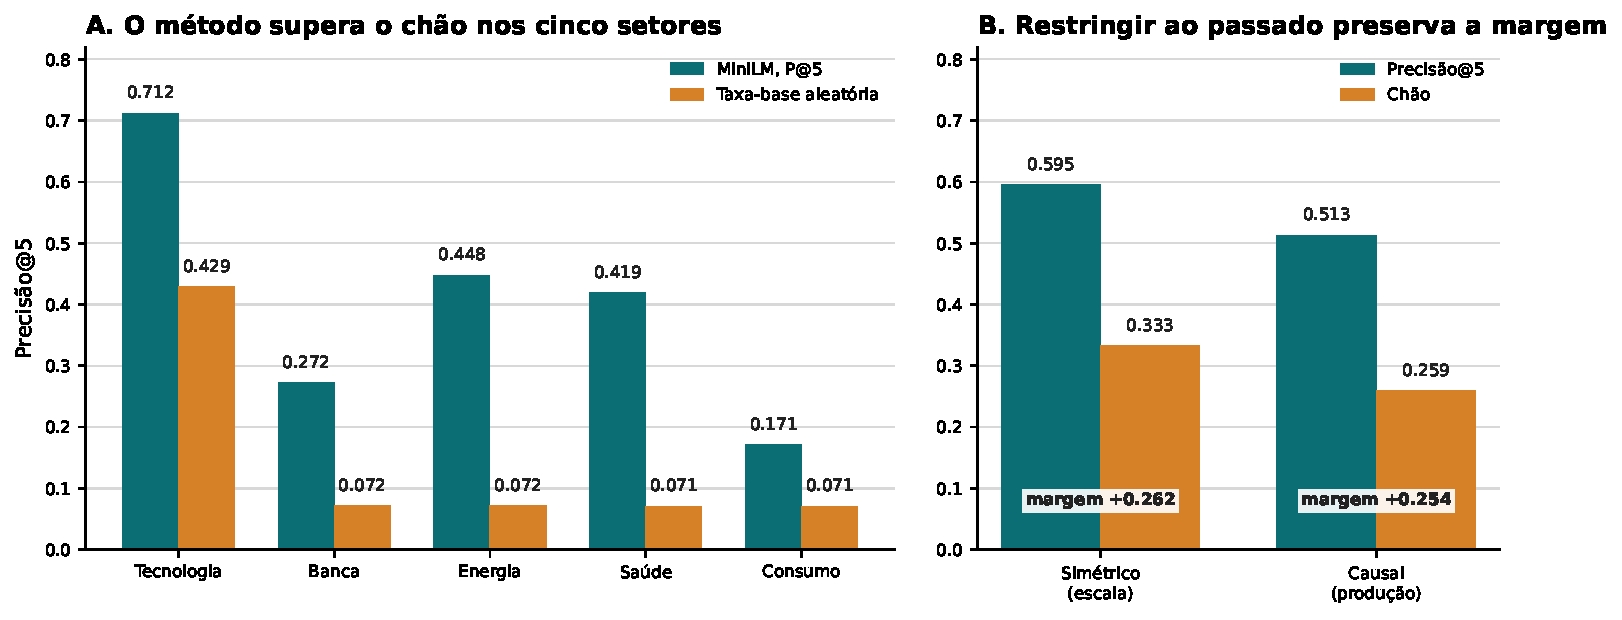
\includegraphics[width=0.96\textwidth]{figures/eval_retrieval_sector_causal.pdf}
\caption[Recuperação por setor e sob a restrição temporal]{À esquerda, precisão@5 do MiniLM e a
taxa-base aleatória dentro de cada setor: o método fica acima do respetivo chão nos cinco. À direita,
o protocolo simétrico de escala e o protocolo causal da produção, cada um ao lado do seu chão. A
precisão baixa de $0.595$ para $0.513$, mas a margem sobre o acaso muda apenas de $+0.262$ para
$+0.254$.}
\label{fig:av_recuperacao}
\end{figure}

E a alternativa que parece mais razoável de todas, ``mostra-me apenas as notícias mais
recentes'', é a \textbf{pior} de todas, com $12.6\%$. Faz sentido: a notícia mais recente sobre
outra empresa não tem razão nenhuma para estar relacionada com esta.

\subsection{Aguenta à escala?}

A avaliação acima corre sobre um corpus recente e curto, pelo que, para confirmar que o resultado
não é um acidente desse corpus, a mesma medição foi repetida sobre o conjunto histórico completo,
com cerca de 80 mil notícias de seis anos. Neste teste de escala \textbf{simétrico}, que ainda
permite candidatos posteriores à consulta, a precisão@5 não só se mantém como sobe, para
$\mathbf{0.595}$.

Convém, no entanto, não ler essa subida como se fosse toda ganho. O chão de acaso também sobe, de
$0.240$ no corpus recente para $0.333$ no completo, porque a mistura de setores é diferente e
acertar por sorte fica mais fácil. Medida contra o respectivo chão, a margem é de $+0.274$ no
primeiro caso e $+0.262$ no segundo, ou seja praticamente a mesma. O que este resultado mostra,
lido com rigor, não é que o método melhore com mais dados: é que \textbf{não se degrada} quando o
corpus passa de recente e curto para seis anos, e era isso que estava em causa.

\subsection{E se o sistema só puder olhar para trás?}
\label{sec:av_qi2_causal}

Há uma liberdade que o protocolo acima permite e que o sistema em produção não tem, e é preciso
dizê-la. A restrição imposta é que a notícia recuperada seja de \emph{outra empresa}, e mais
nada: em particular, ela pode ser \textbf{posterior} à consulta. E não é raro, é o caso comum:
no corpus recente, $38.7\%$ dos vizinhos devolvidos têm data posterior à da consulta e outros
$30.2\%$ são do mesmo dia.

O sistema implantado não tem essa liberdade. A base de precedentes só recebe um caso oito dias
depois, quando o impacto no preço já é observável, portanto tudo o que ele consegue devolver é
passado. O número acima descreve, então, uma tarefa ligeiramente mais fácil do que aquela que o
produto executa, e a pergunta de investigação fala em encontrar notícias \emph{passadas}.

Convém separar duas coisas antes de medir. Isto \textbf{não} é uma fuga de informação no sentido
habitual: o critério de acerto é \emph{pertencer ao mesmo setor}, e o setor de uma notícia não
muda com o tempo, pelo que a direção temporal não tem por onde inflacionar a precisão. O que
está em causa é mais simples: se o número reportado corresponde à tarefa que a pergunta descreve.

A medição repete o protocolo exatamente, acrescentando à máscara a condição de o candidato ser
\textbf{estritamente anterior} à consulta, e reproduz o número simétrico na mesma corrida para a
comparação ser emparelhada. Nenhuma das $2500$ consultas ficou sem passado suficiente. A
Tabela~\ref{tab:av_causal} põe as duas leituras lado a lado.

\begin{table}[ht]
\caption[A recuperação sob a restrição da produção]{A mesma tarefa, com e sem a restrição de o
precedente ter de ser anterior à consulta. A coluna que interessa é a última.}
\label{tab:av_causal}
\centering
\begin{tabular}{l c c c}
\toprule
\tabhead{O que o sistema pode ver} & \tabhead{Precisão@5} & \tabhead{Chão} & \tabhead{Margem} \\
\midrule
Tudo menos a própria empresa & $0.595$ & $0.333$ & $+0.262$ \\
\textbf{Só o que é anterior} & $\mathbf{0.513}$ & $0.259$ & $\mathbf{+0.254}$ \\
\bottomrule
\end{tabular}
\end{table}

A precisão desce $0.082$, o que parece muito. Mas o chão desce quase outro tanto, porque
restringir os candidatos aos anteriores muda a composição do conjunto de onde se escolhe e
acertar por sorte deixa de ser tão provável. Medida contra o respectivo chão, \textbf{a margem
muda $0.008$}: o método mantém praticamente toda a vantagem quando é obrigado a trabalhar como
trabalha em produção.

Repare-se que esta é a \emph{terceira} vez neste capítulo em que ler uma precisão sem
o seu chão daria a conclusão errada. Foi assim na passagem do corpus recente para o completo, foi
assim na precisão dentro do orçamento, onde custou uma afirmação retirada, e é assim aqui.
Não é coincidência: uma precisão é uma quantidade sem significado próprio, e só o adquire ao lado
da alternativa que não sabe nada.

\subsection{O que isto não permite concluir}

Duas observações, e a segunda tem consequências para o produto.

Primeiro, ``mesmo setor'' não é o mesmo que ``relacionado'': é uma aproximação construída porque era
verificável, e não porque fosse exatamente aquilo que se queria medir, e o número deve ser lido com
essa reserva.

Segundo, e mais interessante: a recuperação capta \textbf{tema}, não \textbf{direção}. Duas notícias
podem ser sobre o mesmo assunto e o preço ter ido para lados opostos, que foi exatamente o que
aconteceu no exemplo do Capítulo~\ref{cap:sistema}. Medindo a concordância de direção entre a
notícia de consulta e os casos recuperados, obtém-se $0.708$ contra um chão de acaso de $0.688$: quase
nada. Daí que o sistema mostre os casos um a um e nunca os resuma a uma média, e daí também que o texto do
alerta diz explicitamente que se trata de casos semelhantes no \emph{tema}.

\section{QI3: decidir o que merece um alerta}
\label{sec:av_qi3}

\emph{Um modelo treinado prioriza notícias melhor do que uma linha de base simples baseada só em
volatilidade?} \textbf{Não. E é o resultado mais interessante deste trabalho.}

\subsection{Como foi medido}

O conjunto de dados foi construído a partir do histórico: \textbf{79\,753} exemplos entre 2018 e
2023, cada um uma notícia com o contexto de mercado do dia e o rótulo descrito na
Secção~\ref{sec:met_triagem}. A divisão é cronológica com embargo, como na
Figura~\ref{fig:divisao}.

O protocolo é causal em relação aos dias posteriores, mas uma entrada não está disponível no mesmo
referencial em produção: \texttt{ret\_event} é o retorno completo do dia $d$ no conjunto offline e
a notícia é pontuada antes desse dia fechar. Por isso, o resultado abaixo avalia o modelo com a
variável diária completa; não demonstra paridade com a pontuação intradiária. A
Secção~\ref{sec:av_ret_event_producao} mede o sintoma em produção e separa o que os registos permitem
concluir.

Convém dizer para que lado essa assimetria empurra, porque não é neutra e porque é a primeira
objeção que a secção levanta. A entrada \texttt{ret\_event} pertence ao bloco de contexto, ou seja
está nos modelos que \emph{perdem}; a linha de base vencedora usa uma única entrada, a volatilidade
dos vinte dias anteriores, e essa está fechada na véspera. O referencial mais generoso está portanto
do lado dos modelos que a comparação não favorece, e corrigi-lo só poderia tornar o resultado
negativo mais forte, nunca mais fraco. O que fica por demonstrar é o nível das métricas, e não a
ordenação entre as famílias.

Compararam-se seis modelos, do mais simples ao mais completo. A métrica principal é a
\textbf{PR-AUC}, apropriada quando as duas classes são desequilibradas.

Para efeitos práticos, uma diferença de PR-AUC abaixo de $0.02$ é tratada como indistinguível,
mesmo quando o intervalo emparelhado exclui zero. O limite é uma escolha do autor; declará-lo aqui,
antes dos resultados, obriga a aplicá-lo nos dois sentidos.

Dois cuidados de montagem, ambos para que a comparação não favoreça a conclusão que se acabou por
obter. Primeiro, um dos seis modelos é um conjunto de árvores treinado por reforço do gradiente
\autocite{friedman2001gbm}, incluído por ser o mais expressivo dos seis: capta interações e efeitos
não lineares entre as variáveis que a regressão logística, por construção, não capta.
Com uma ressalva que enfraquece a palavra \emph{teto} e que é preciso dar: correu com os
parâmetros por defeito da biblioteca, sem qualquer procura de hiperparâmetros. Um modelo de
árvores por afinar não é o melhor que essa família consegue, portanto a sua derrota limita o que
se pode concluir: mostra que o texto não aparece \emph{nesta} montagem, e não que não apareceria
num modelo não linear bem afinado. Serve de teto,
e se o texto tivesse sinal a extrair era ali que teria mais hipóteses de aparecer. Convém enunciar o
alcance exato desta garantia: mostra que \emph{nenhum dos seis} modelos comparados extraiu sinal do
texto, e não que nenhum modelo o conseguiria. Um método mais recente, ou o corpo dos artigos em vez
do título, continuam por testar. Segundo, todas as pontuações são convertidas em probabilidades por calibração
\emph{a posteriori} sobre um bloco de validação reservado \autocite{niculescu2005calibration}, sem o
que a coluna do Brier não seria comparável entre modelos.

\subsection{Resultado}

\begin{table}[ht]
\caption[Triagem: seis modelos sobre o mesmo bloco de teste]{Quanto maior a PR-AUC, melhor; quanto
menor o Brier, melhor calibradas estão as probabilidades.}
\label{tab:av_triagem}
\centering
\begin{tabular}{l c c}
\toprule
\tabhead{Modelo} & \tabhead{PR-AUC} & \tabhead{Brier} \\
\midrule
Alertar sempre (chão) & $0.378$ & $0.622$ \\
\textbf{Só volatilidade} & $\mathbf{0.542}$ & $\mathbf{0.218}$ \\
Só contexto de mercado & $0.538$ & $0.224$ \\
Só texto do título & $0.439$ & $0.240$ \\
Contexto $+$ texto & $0.496$ & $0.229$ \\
Árvores com reforço do gradiente (contexto $+$ texto) & $0.469$ & $0.228$ \\
\bottomrule
\end{tabular}
\end{table}

A Figura~\ref{fig:av_triagem} mostra as curvas completas, e não apenas o número resumo.

\begin{figure}[ht]
\centering

\includegraphics[width=0.86\textwidth]{figures/eval_triage_pr.pdf}
\caption[As curvas de precisão e cobertura da triagem]{As curvas sobre o bloco de teste. A área
debaixo de cada curva é o valor da tabela. A curva do modelo que usa apenas volatilidade está por
cima das outras em quase toda a extensão, e não só no valor agregado.}
\label{fig:av_triagem}
\end{figure}

O melhor modelo da Tabela~\ref{tab:av_triagem} é o mais simples de todos: o que usa \textbf{apenas a volatilidade
recente}. Acrescentar o resto do contexto não melhora. Acrescentar o texto do título
\emph{piora}, de $0.542$ para $0.496$.

Isto era o contrário do que eu esperava quando comecei. A hipótese era que o texto da notícia
trouxesse informação que os preços não tinham. Sobre este corpus, não traz.

\subsection{Não será um acidente da minha montagem?}

Foi a primeira hipótese que fui verificar, por três caminhos.

\paragraph{Será que o modelo de texto estava mal afinado?} Repetiu-se a comparação dando ao texto as
melhores condições possíveis: regularização afinada, redução do bloco de texto a $32$ dimensões, e
um modelo de linguagem especializado em finanças. O melhor resultado do texto sobe para $0.533$,
e continua abaixo dos $0.542$ da volatilidade.

\paragraph{Será que a diferença é ruído?} Reamostrou-se o bloco de teste mil vezes, por grupos
(empresa, dia), porque notícias do mesmo dia sobre a mesma empresa partilham o rótulo e não são
observações independentes. A diferença mantém-se com o intervalo a excluir zero.

\textbf{E convém dizer a que pergunta este intervalo responde, porque não é a mais larga.} A
reamostragem é feita \emph{dentro} de um único bloco de teste, que são $221$ dias de negociação;
mede portanto o ruído de amostragem nesse período e não diz nada sobre a estabilidade entre
períodos. A distinção não é teórica neste trabalho: a Secção~\ref{sec:av_deriva} mede um
\gls{PSI} de $0.281$ na volatilidade, e a prevalência do rótulo passa de $47.0\%$ na validação
para $37.8\%$ no teste. Se a variação de um período para outro é dessa ordem, é plausível que a
variância \emph{entre} janelas seja maior do que os efeitos que aqui se declaram distinguíveis de
zero, e todas as comparações deste capítulo, incluindo as nove definições de rótulo e as
ablações, correm sobre o mesmo bloco. Uma origem rolante com três ou quatro cortes sucessivos
responderia à pergunta larga, e não foi feita; fica declarado, e não contornado.

\paragraph{Será que depende de como defini o rótulo?} O rótulo usa um limiar de $2\%$ e um horizonte
de três dias, ambos escolhidos por mim. Repetiu-se toda a comparação para nove combinações
diferentes de limiar e horizonte. A volatilidade iguala ou bate o modelo com texto nas
\textbf{nove}.

O resultado negativo aguenta os três testes. Não é um acidente da minha montagem: é o que os dados dizem.

\paragraph{E há uma quarta verificação, que fiz por último e que corta nos dois sentidos.}
Contei quantas empresas há em cada bloco, coisa que a divisão cronológica não garante, e os três
blocos \textbf{quase não partilham empresas}. O treino vai de 2018-01-02 a 2022-03-03 e tem treze
nomes; o teste vai de 2023-02-02 a 2023-12-18 e tem nove. Cinco empresas do treino não aparecem
uma única vez no teste, e uma empresa do teste, que vale $17.1\%$ das suas linhas, nunca aparece
no treino. Pior: para as que estão nos dois lados, a taxa de positivos desloca-se muito, e a
Apple passa de $0.448$ no treino para $0.183$ no teste. Isto lê-se direto das colunas
\texttt{split} e \texttt{ticker} do conjunto congelado e não precisa de nenhuma corrida nova.

Não é uma fuga nem um erro de divisão: o corte é por dia, e por dia a proporção é a que a
Secção~\ref{sec:met_split} declara. É a composição do corpus que muda com o tempo, pela mesma razão
que ali torna o bloco de teste maior do que o de treino --- as empresas de que se escreve em 2018
não são as de que se escreve em 2023.

E a consequência puxa nos dois sentidos, por isso fica escrita inteira. \textbf{A favor do
resultado negativo:} um modelo cujo sinal é, no essencial, a identidade da empresa
(Secção~\ref{sec:av_ablacao}) está a estimar essa identidade sobre um conjunto de empresas que mal
existe no bloco onde é avaliado, ao passo que a volatilidade é medida no próprio dia e atravessa
empresas. Isso é uma explicação adicional, e mais concreta do que a que eu tinha, para a linha de
base ganhar. \textbf{Contra:} também quer dizer que a comparação não separa \emph{o modelo é pior}
de \emph{a identidade não transfere entre estes dois períodos}, e essa separação exigiria uma
divisão que mantivesse a composição constante --- que não foi feita. Também explica, sem
recorrer ao acaso, a prevalência de $47.0\%$ da validação contra $37.8\%$ do teste: são conjuntos
de empresas diferentes, e não apenas períodos diferentes.

\subsection{Mas tem utilidade prática?}

Serve, mas aqui é preciso muito cuidado com a comparação, porque é fácil enganar-se.

O produto não mostra tudo: mostra no máximo cinco alertas por dia. A pergunta útil passa a ser
A Tabela~\ref{tab:av_orcamento} responde.

\begin{table}[ht]
\caption[Precisão dentro de um orçamento de cinco alertas por dia]{Quatro formas de escolher as cinco
notícias do dia, sobre o mesmo bloco de teste. As quatro escolhem \emph{sabendo o dia inteiro}, e
por isso os valores são limites superiores do que uma política online consegue: ver a ressalva na
Secção~\ref{sec:av_qi3}.}
\label{tab:av_orcamento}
\centering
\small
\begin{tabular}{l c p{0.42\textwidth}}
\toprule
\tabhead{Como escolher} & \tabhead{Precisão@5} & \tabhead{O que é} \\
\midrule
``Alertar sempre'' & $0.163$ & \emph{não é escolher às cegas}; ver o aviso abaixo \\
Ao acaso (40 sementes) & $0.379 \pm 0.017$ & o que ``às cegas'' quer mesmo dizer \\
Volatilidade média da empresa & $\mathbf{0.662}$ & treze constantes, sem ler título nenhum \\
O modelo treinado & $0.632$ & o que está implantado \\
\bottomrule
\end{tabular}
\end{table}

\begin{tcolorbox}[colback=orange!5, colframe=orange!45, boxrule=0.5pt, arc=2pt]
\textbf{Um aviso sobre a primeira linha, que eu próprio quase publiquei errado.} O modelo
``alertar sempre'' dá a mesma pontuação a todas as notícias. Quando todas empatam, a métrica escolhe
pela ordem em que as linhas aparecem no ficheiro, e o ficheiro está ordenado por data e por nome
da empresa. Ou seja, esse $0.163$ \textbf{não mede escolher ao acaso: mede escolher por ordem
alfabética}, e todas as linhas que ele seleciona pertencem à empresa que vem primeiro no alfabeto.

Comparado com o chão certo, o ganho do modelo é de $1.67$ vezes, e não das quase quatro vezes que a
primeira leitura sugeria. Deixo isto escrito porque foi um erro meu, e porque a lição é geral:
\emph{verificar o que a linha de base mede é tão importante como verificar o que o modelo faz}.
\end{tcolorbox}

Há ainda a terceira linha, que é desconfortável e fica. Uma tabela de \textbf{treze constantes},
a volatilidade média de cada empresa, calculada só sobre o bloco de treino e sem ler um único
título, obtém $0.662$ e \textbf{bate o modelo treinado}. É o terceiro caso deste capítulo em que o
método mais simples ganha. O que a evidência sustenta, portanto, é
que \emph{ordenar por volatilidade} compensa; não que \emph{aprender} compense.

\subsection{E em produção?}

O sistema regista todas as decisões de triagem e, dias depois, verifica o que realmente aconteceu.
Sobre $825$ decisões já maturadas, o modelo não mostra benefício: as notícias que ele deixou passar
eram importantes $58.9\%$ das vezes, contra $61.7\%$ das que ele travou.

Estes dois números pedem uma ressalva sobre a sua precisão, e ela é grande. As $825$ decisões não
são $825$ observações independentes: o rótulo é atribuído por \emph{(empresa, dia)}, e as $825$
linhas repartem-se por apenas $239$ pares distintos. Medida sobre essas $239$ unidades, a capacidade
de ordenação do modelo, a \textbf{\gls{ROCAUC}}, fica em $0.486$ com um intervalo de confiança a
$95\%$ de $[0.403, 0.571]$. Nesta medida o acaso vale exatamente $0.5$, portanto o intervalo
contém-no confortavelmente. A leitura correta não é que o modelo seja pior do que
nada, mas que \textbf{esta amostra não distingue o modelo do acaso}.

\paragraph{E duas das doze empresas vigiadas não estão no corpus de treino.}
O mapa canónico do material histórico tem quinze nomes, o conjunto de dados construído cobre
catorze e o \emph{bloco de treino} cobre treze --- que é a razão de a tabela de consulta da
Secção~\ref{sec:av_ablacao} ter treze constantes e não catorze; a lista que o
produto vigia tem doze, e duas delas nunca apareceram em nenhum exemplo de treino. O modelo
pontua-as na mesma, porque o que ele recebe são valores numéricos e não a identidade da empresa,
mas fá-lo sobre uma combinação de entradas que não viu. É um segundo sentido, mais literal, em que
o modelo implantado corre fora da distribuição em que foi avaliado, e as decisões dessas duas
empresas entram nas $825$ acima como quaisquer outras.

Esta medição foi refeita a 20 de agosto de 2026, quando o registo já tinha $825$ decisões
maturadas contra as $530$ de que dispunha a primeira leitura. Vale a pena dizer o que mudou,
porque quase nada mudou: a diferença entre mantidas e suprimidas estreitou-se (era $59.2\%$
contra $64.7\%$), a \textbf{ROC-AUC} passou de $0.494$ para $0.486$, e o intervalo encolheu.
Com metade mais evidência o veredicto é o mesmo, e é mais firme.

A explicação mais provável não é que o modelo esteja avariado, mas que esteja a \textbf{mais}.
Quando ele é chamado, as notícias já passaram pelo filtro de relevância e pelo de frescura. Esses
filtros baratos já removeram grande parte do que o modelo foi treinado para remover, e sobra-lhe
pouco para separar. \textbf{Um modelo avaliado isolado e implantado atrás de filtros nunca foi
avaliado na distribuição que vai ver.} É a lição mais transferível deste trabalho.

\subsection{E os dados de hoje ainda se parecem com os do treino?}
\label{sec:av_deriva}

Há uma segunda razão pela qual um modelo implantado pode deixar de servir, e é independente da
anterior: os dados mudam. Este foi treinado sobre 2018--2023 e corre em 2026. A distância está
afirmada em vários sítios deste documento, e afirmar é barato, portanto foi medida.

A medida usada é o \gls{PSI}, que compara a distribuição de cada entrada entre o período de treino
e o atual, com as bandas convencionadas em risco de crédito: abaixo de $0.10$ estável, entre
$0.10$ e $0.25$ moderada, acima de $0.25$ significativa.

O resultado tem duas metades e as duas interessam. A entrada que mais se deslocou é a
\textbf{volatilidade dos vinte dias anteriores}, com \gls{PSI} de $0.281$, ou seja na banda
significativa; as restantes ficam estáveis. Mas o \textbf{rótulo quase não se move}: a prevalência
de positivos passa de $0.3854$ para $0.3781$.

É uma combinação incómoda de ler e vale a pena dizer o que significa. A entrada de que o modelo mais
depende é precisamente a que mais derivou, e o que ele tenta prever manteve-se onde estava. Não
invalida nenhum número deste capítulo, porque todos foram medidos dentro do mesmo período, mas
diz que o modelo implantado está a ver uma distribuição que já não é a do treino. Aqui a deriva é
\textbf{medida e não corrigida}: nada se re-treina, e a Secção~\ref{sec:con_futuro} diz o que
faria falta para isso.

\subsection{E o que é que a porta estava a escolher, afinal?}
\label{sec:av_portao}

A subsecção anterior diz que o modelo está \emph{a mais}. Serve de explicação e é vaga: não
diz \textbf{o que} ele estava a fazer quando era chamado. Vale a pena responder a isso, porque a
resposta é medível e porque foi ela que mudou o sistema.

A pergunta é simples. A porta implantada era um limiar fixo sobre a probabilidade calibrada: passa
quem estiver acima de $0.50$. \emph{Esse limiar separava títulos, ou separava empresas?}

Mediu-se sobre as $4\,366$ decisões \textbf{realmente tomadas em produção}, e a
Figura~\ref{fig:av_portao} mostra o resultado de uma só vez.

\begin{figure}[ht]
\centering
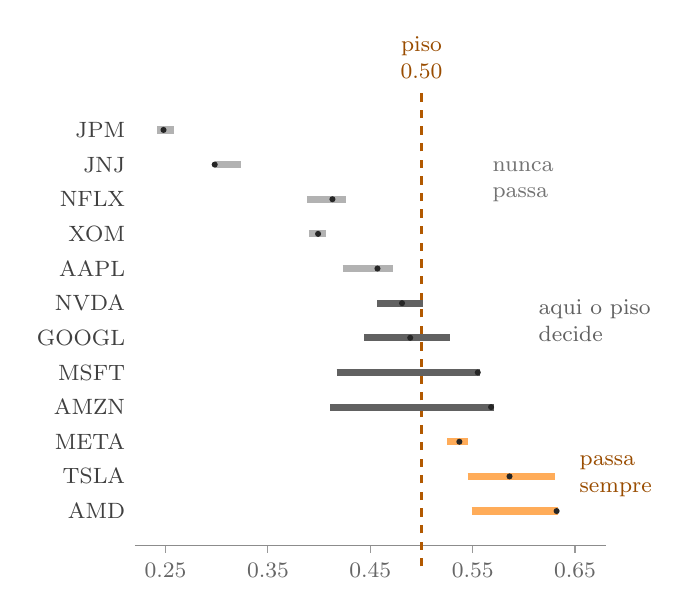
\begin{tikzpicture}[font=\footnotesize, x=13cm, y=0.44cm]
  % eixo
  \draw[black!45] (0.22,0) -- (0.68,0);
  \foreach \x in {0.25,0.35,0.45,0.55,0.65}
    \draw[black!40] (\x,0) -- (\x,-0.22) node[below, black!60] {\x};
  % o piso
  \draw[dashed, thick, orange!70!black] (0.50,-0.6) -- (0.50,13.2)
    node[above, align=center, text=orange!60!black] {piso\\ $0.50$};
  % (linha, ticker, mínimo, mediana, máximo, COR). A cor vai nos dados de propósito: uma
  % condicional dentro do \foreach falha em silêncio e as barras saem todas iguais.
    % Variaveis do \foreach nunca podem chamar-se \c \t \l \i \o: sao comandos do
  % LaTeX (cedilha, til, l barrado, i sem ponto, o barrado) e o \foreach substitui-os
  % tambem DENTRO das palavras. Ver a Figura 6.1, onde \c transformava "avaliacao"
  % em "avalia<custo>cao" sem um unico aviso de compilacao.
  \foreach \xn/\xtk/\xa/\xm/\xb/\xcor in {
    12/JPM/0.242/0.248/0.258/black!30, 11/JNJ/0.298/0.298/0.324/black!30,
    10/NFLX/0.388/0.413/0.426/black!30, 9/XOM/0.390/0.399/0.407/black!30,
    8/AAPL/0.423/0.457/0.472/black!30, 7/NVDA/0.457/0.481/0.501/black!62,
    6/GOOGL/0.444/0.489/0.528/black!62, 5/MSFT/0.417/0.555/0.557/black!62,
    4/AMZN/0.411/0.568/0.571/black!62, 3/META/0.525/0.537/0.545/orange!65,
    2/TSLA/0.545/0.586/0.630/orange!65, 1/AMD/0.549/0.632/0.633/orange!65}
  {
    \node[left, black!75] at (0.22,\xn) {\xtk};
    \draw[line width=2.6pt, color=\xcor] (\xa,\xn) -- (\xb,\xn);
    \fill[black!85] (\xm,\xn) circle (1.1pt);
  }
  \node[right, align=left, text=orange!60!black] at (0.645,2) {passa\\ sempre};
  \node[right, align=left, black!55] at (0.56,10.5) {nunca\\ passa};
  \node[right, align=left, black!62] at (0.605,6.5) {aqui o piso\\ decide};
\end{tikzpicture}
\caption[O que a porta separava]{Para cada empresa, o intervalo de todas as pontuações que o
modelo lhe deu em produção, com a mediana marcada a preto. A linha tracejada é o piso de decisão.
As barras claras nunca o alcançam, as escuras atravessam-no, e as alaranjadas estão sempre acima.
Repare-se em que oito das doze estão \textbf{inteiramente} de um dos lados: para essas, a decisão
estava tomada antes de se ler o título.}
\label{fig:av_portao}
\end{figure}

A leitura da figura é imediata e os números confirmam-na:

\begin{itemize}
  \item a amplitude média das pontuações \textbf{dentro} de cada empresa é $0.064$;
  \item a amplitude \textbf{entre} as medianas das empresas é $0.385$, ou seja, $6.1$ vezes maior;
  \item três empresas ficavam \textbf{sempre} acima do piso e cinco \textbf{nunca} lá chegavam;
  \item só em quatro das doze o piso decidia alguma coisa.
\end{itemize}

\begin{tcolorbox}[colback=orange!5, colframe=orange!45, boxrule=0.5pt, arc=2pt]
Em \textbf{$48\%$} dos títulos distintos --- e em $84\%$ das decisões registadas, que é a
contagem mais generosa das duas e está discutida a seguir --- o resultado estava determinado pela
\textbf{empresa} antes de o título ser lido. A Apple não conseguia gerar um alerta de notícia,
acontecesse o que acontecesse; a AMD passava em $963$ de $963$.
\end{tcolorbox}

As duas contagens medem coisas diferentes e ambas ficam. O sistema repontua os mesmos títulos a
cada ciclo de sessenta segundos, e a duplicação é maior nas empresas com menos notícias, que são
as que nunca passam o piso; contar decisões empurra portanto a fração para cima. Contado uma vez
por título distinto, sobre uma janela maior de $36\,925$ decisões, a fração é de $48\%$. A
conclusão estrutural não depende de qual se escolha: continua a haver empresas inteiramente de um
dos lados do piso, e a amplitude entre empresas continua a ser várias vezes a amplitude dentro de
cada uma.

O defeito tem a mesma forma que o da Secção~\ref{sec:av_qi1}, uma camada acima: aí, um limiar fixo
sobre o retorno mede a volatilidade da empresa em vez da raridade do dia; aqui, um limiar fixo
sobre uma pontuação quase constante por empresa ordena empresas em vez de notícias.

Nenhum teste o podia detetar. O modelo foi avaliado sobre a distribuição do conjunto de treino e
implantado atrás de dois filtros que a alteram, e cada peça cumpria o seu contrato: o que estava
errado era uma suposição sobre a ligação entre elas, não escrita em lado nenhum. É a classe de
custo que \textcite{sculley2015debt} arrumam sob dependências de dados e emaranhamento entre
componentes, com o sintoma que eles descrevem: o sistema continua a produzir números de aparência
normal.

\paragraph{E há uma segunda causa possível, que não consigo separar da primeira.}
\label{sec:av_ret_event_producao}
Uma das nove entradas do modelo é a \textbf{reação do próprio dia}, e no treino ela é o retorno do
fecho de $d-1$ para o fecho de $d$, ou seja o movimento completo do dia da notícia, que só se
conhece quando esse dia fecha. Em produção o sistema pontua a notícia no minuto em que a apanha,
com uma latência mediana de $158$ minutos desde a publicação e exemplos captados às
$08{:}14$: a essa hora o dia da notícia ainda não fechou. A entrada é então calculada sobre a
última barra diária que a fonte tem, que durante a sessão é o fecho da véspera ou uma barra
incompleta do próprio dia. Em nenhum dos casos é a quantidade sobre a qual o modelo foi treinado.

As duas causas produzem o mesmo sintoma e o registo não permite atribuir peso a cada uma, porque
guarda a probabilidade e o resultado mas não o valor das entradas no momento da pontuação.
Separá-las exigiria registar essas entradas e voltar a observar durante semanas.

\subsection{E a medição acima não é uma surpresa: é aritmética}
\label{sec:av_inevitavel}

Apresentei o resultado anterior como uma descoberta empírica. Ao verificá-lo percebi que é pior do
que isso, e é preciso dizê-lo com clareza porque muda a leitura.

O modelo implantado é a variante \textbf{sem texto}. Como a Secção~\ref{sec:met_modelo_ve} já
mostrou, das suas entradas apenas uma distingue dois títulos da mesma empresa no mesmo dia: o
comprimento do título. Com o peso que essa entrada tem, oitenta caracteres a mais deslocam a
pontuação interna do modelo em $0.0128$, e depois de passar pela calibração isso são poucos
milésimos na probabilidade que o sistema mostra. A amplitude entre empresas, medida nessa mesma
probabilidade, é de $0.385$. As duas grandezas separam-se por duas ordens de magnitude.

O cuidado com as escalas é deliberado e vale a pena explicá-lo, porque é fácil enganar-se aqui: o
$0.0128$ vive na escala interna do modelo, antes da calibração, e o $0.385$ vive na probabilidade
calibrada. Pô-los lado a lado sem os converter compararia coisas diferentes, e a conversão só torna
o argumento mais forte, não mais fraco.

\begin{tcolorbox}[colback=orange!5, colframe=orange!45, boxrule=0.5pt, arc=2pt]
A pontuação quase constante dentro de cada empresa não é um acidente do treino nem um defeito dos
dados. É uma \textbf{consequência aritmética do conjunto de entradas}. O modelo implantado nunca
foi capaz de ordenar notícias, e nenhum treino o tornaria capaz.
\end{tcolorbox}

Isto podia ficar-se por um raciocínio sobre a lista de entradas, e um raciocínio não é uma prova.
Vale a pena testá-lo, e o teste é o mais simples possível.

\subsection{A prova: uma tabela que não vê a notícia}
\label{sec:av_ablacao}

Se o modelo aprendeu sobretudo a reconhecer a empresa, então deve ser possível reproduzi-lo com
uma \textbf{tabela de consulta}: para cada empresa, um único número fixado no bloco de treino, que
é a fração das suas notícias que se revelaram importantes. Essa tabela não vê o título, não vê o
dia, não vê nada. Devolve sempre o mesmo valor para a mesma empresa.

A Tabela~\ref{tab:av_ablacao} compara-a com o modelo implantado e desmonta o modelo entrada a
entrada, tudo sob o protocolo congelado.

\begin{table}[ht]
\caption[O modelo, desmontado entrada a entrada]{Cada linha é um modelo treinado com menos
informação do que o anterior. A terceira linha é a decisiva: não vê a notícia e iguala o modelo
implantado.}
\label{tab:av_ablacao}
\centering
\small
\begin{tabular}{L{0.34\textwidth} L{0.30\textwidth} C{0.11\textwidth} C{0.13\textwidth}}
\toprule
\tabhead{Modelo} & \tabhead{O que vê} & \tabhead{PR-AUC} & \tabhead{Precisão@5} \\
\midrule
Contexto completo (o implantado) & as nove entradas & $0.538$ & $0.632$ \\
Só volatilidade & uma entrada, de empresa & $0.542$ & $0.632$ \\
\midrule
\textbf{Tabela de consulta por empresa} & \textbf{nada da notícia} & $\mathbf{0.534}$ &
$\mathbf{0.662}$ \\
\midrule
Sem os indicadores de setor & tira 5 entradas de empresa & $0.543$ & $0.629$ \\
Sem volatilidade nem momento & tira as 2 que restam & $0.389$ & $0.390$ \\
Sem nada de nível de empresa & fica o dia e a notícia & $0.378$ & $0.368$ \\
Só o comprimento do título & a única de nível de notícia & $0.378$ & $0.352$ \\
\bottomrule
\end{tabular}
\end{table}

Três leituras, e nenhuma delas depende de interpretação.

\paragraph{A tabela de consulta iguala o modelo, e numa das métricas bate-o.}
Na PR-AUC obtém $0.534$ contra $0.538$, uma diferença de $0.004$. Na precisão dentro do orçamento,
que é a métrica mais próxima do uso real, obtém $0.662$ contra $0.632$, ou seja \textbf{fica à
frente}. Um número por empresa, fixado meses antes e nunca atualizado, faz o mesmo que o modelo
treinado e, no critério que mais se parece com o produto, faz melhor.
\textbf{O modelo implantado é uma tabela de consulta.}

\paragraph{Sem a empresa, não sobra nada.}
Retirando todas as entradas de nível de empresa, a PR-AUC cai para $0.378$, que é precisamente a
prevalência do bloco de teste, ou seja, o chão definido na Secção~\ref{sec:av_prauc}. Um modelo que
obtém exatamente o chão não aprendeu nada.

\paragraph{E a única entrada que descreve a notícia não acrescenta nada.}
O comprimento do título, sozinho, também dá $0.378$ de PR-AUC. É o mesmo chão. A única informação
por título que o modelo implantado recebia é indistinguível de não receber informação nenhuma.

Isto obriga a separar duas afirmações que eu tinha juntado, e a separação é a parte honesta:

\begin{itemize}
  \item \textbf{A conclusão científica da \gls{QI}3 mantém-se.} A variante \emph{com} texto tem
        $384$ números por título, portanto tem mesmo informação sobre a notícia, e ainda assim
        obteve $0.496$ contra os $0.542$ da volatilidade. É essa comparação que responde à
        pergunta, e o resultado negativo é dela.
  \item \textbf{A decisão de produto estava errada por outra razão.} O que foi implantado como
        porta de decisão foi a variante \emph{sem} texto, e escolhi-a sem reparar que a métrica
        que usei para o fazer não fazia a pergunta de que o produto precisava.
\end{itemize}

\paragraph{Porque se manteve a variante de nove entradas.}
Não foi por ter a melhor PR-AUC entre as que cabiam no contentor: só volatilidade obtém $0.542$ e
sem os indicadores de setor $0.543$, contra $0.538$, e ambas cabiam. A razão defensável é a
explicabilidade: só a variante de nove entradas permite ao alerta mostrar contribuições que sobem e
descem a pontuação (Figura~\ref{fig:sis_alerta}). O preço dessa escolha é $0.005$ de PR-AUC.

A lição de método mantém-se: a PR-AUC sobre o conjunto inteiro pode ser alta quando a variação
\emph{entre} empresas domina, mesmo sem distinguir notícias dentro da mesma empresa. A métrica
respondia a \emph{ordena bem o conjunto?}; o produto precisava de \emph{distingue duas notícias da
mesma empresa?}.

\subsection{E se o texto não for para substituir, mas para acrescentar?}
\label{sec:av_acrescimo}

Comparar só volatilidade, só contexto e só texto responde a \emph{qual é melhor}; não responde a
\emph{o texto acrescenta informação}. Para o testar é preciso somá-lo a uma base que conheça a
empresa sem conhecer a notícia.

A variante \emph{contexto + texto} parece já fazer isso, e não faz, por uma razão que a
Secção~\ref{sec:av_ablacao} tornou visível: soma o texto ao bloco de contexto, que \textbf{não é}
a base certa para esta pergunta. A base certa é a \textbf{tabela de consulta por empresa}, e a
razão é metodológica e não de desempenho: ela contém tudo o que o modelo sabe sobre a
\emph{empresa} e absolutamente nada sobre a \emph{notícia}, portanto somar-lhe o título isola a
contribuição do texto. Convém dizer o que ela não é: na PR-AUC a volatilidade sozinha fica
\textbf{acima} dela, $0.542$ contra $0.534$, e é por isso que a tabela dos intervalos tem uma
segunda linha. Nunca se tinha testado o texto por cima desta base.

\paragraph{O critério, fixado antes de medir.} Um acréscimo só conta se o intervalo de confiança
a $95\%$ da diferença, obtido por reamostragem \textbf{por grupos} (empresa, dia), excluir zero. E
a representação de texto não foi afinada aqui: usa-se a mesma redução a $32$ dimensões do
re-teste da Secção~\ref{sec:av_qi3}, para que a comparação não seja o resultado de procurar a
configuração que convém.

\begin{table}[ht]
\caption[O texto por cima da tabela de consulta]{Somar o título à tabela de consulta. A coluna
da direita é a capacidade de ordenar \emph{dentro} de cada empresa, onde a tabela vale $0.5$ por
construção e não por estimativa. \textbf{As linhas com texto não são as da
Tabela~\ref{tab:av_triagem} e não devem ser lidas contra ela:} aqui o bloco de texto está reduzido
a $32$ dimensões, como no re-teste favorável ao texto, e é por isso que ``contexto + texto'' dá
$0.533$ aqui e $0.496$ ali. A redução é a mesma para todas as linhas desta tabela, logo a
comparação \emph{dentro} dela é justa.}
\label{tab:av_acrescimo}
\centering
\small
\begin{tabular}{L{0.40\textwidth} C{0.13\textwidth} C{0.13\textwidth} C{0.17\textwidth}}
\toprule
\tabhead{Modelo} & \tabhead{PR-AUC} & \tabhead{Prec.@5} & \tabhead{AUC dentro} \\
\midrule
Tabela de consulta por empresa & $0.534$ & $\mathbf{0.662}$ & $0.500$ \\
\textbf{Tabela + texto} & $\mathbf{0.547}$ & $\mathbf{0.662}$ & $0.512$ \\
Contexto (o implantado) & $0.538$ & $0.632$ & $0.502$ \\
Contexto + texto & $0.533$ & $0.627$ & $0.508$ \\
Só texto & $0.457$ & $0.616$ & $0.495$ \\
\bottomrule
\end{tabular}
\end{table}

\paragraph{O resultado é detetável, mas pequeno.} O título \textbf{acrescenta} a essa base:
$+0.012$ de PR-AUC, com intervalo $[+0.004,\ +0.020]$, que exclui zero. É a primeira vez que uma
representação de texto mostra um acréscimo detetável nesta tarefa, mas fica abaixo do critério
prático de $0.02$ fixado antes dos resultados e não altera a precisão dentro do orçamento.

Três ressalvas impedem que isto seja mais do que é, e todas são medições e não modéstia.

\begin{description}
  \item[Não bate a volatilidade sozinha.] O $0.547$ é maior do que o $0.542$, mas a diferença
        entre os dois tem intervalo $[-0.032,\ +0.037]$, que contém zero. São dois pontos dentro
        do ruído um do outro, e afirmar que o modelo com texto \emph{ganha} seria ler uma
        diferença que esta amostra não sustenta. O veredicto da \gls{QI}3 não muda.

  \item[Não chega ao produto.] A precisão dentro do orçamento de cinco alertas por dia é
        $0.662$ com e sem o texto, sem uma casa decimal de diferença. O acréscimo existe na
        ordenação do conjunto todo e desaparece quando só se escolhem cinco por dia, que é
        exatamente o que o sistema faz. Um ganho que não sobrevive à métrica de produto não muda
        o produto.

  \item[E continua a não separar dias da mesma empresa.] A última coluna da
        Tabela~\ref{tab:av_acrescimo} mede a capacidade de ordenar \emph{dentro} de cada empresa,
        onde a tabela de consulta vale $0.500$ por construção, por devolver sempre o mesmo valor.
        O modelo implantado obtém $0.502$ com intervalo $[0.462,\ 0.542]$, que contém $0.5$; com
        texto sobe para $0.512$, e o acréscimo tem intervalo que também contém zero. Ou seja: a
        informação que o texto traz distingue \textbf{empresas e períodos}, e não notícias. O
        diagnóstico da secção anterior sai confirmado, não desmentido.
\end{description}

\paragraph{O que isto muda na resposta à \gls{QI}3.} A resposta continua a ser não, e passa a ser
mais precisa. Antes dizia-se: \emph{nenhum modelo com texto bate a volatilidade}. Continua
verdade. Acrescenta-se agora: \emph{mas o texto não é inútil}, acrescenta ao que o modelo já sabe
sobre a empresa, de forma pequena e mensurável, e o que o impede de mudar o sistema não é a
ausência de informação, é a informação ser do tipo errado. Distingue empresas quando o produto precisa de
distinguir notícias.

O limite fica assim localizado: o trabalho seguinte pede um rótulo por notícia, não apenas um
modelo maior.

\paragraph{Uma ressalva sobre o próprio método.} Este é mais um modelo avaliado sobre o mesmo
bloco de teste, que já serviu várias comparações deste capítulo. Quanto mais vezes se olha para um
conjunto de teste, mais fácil é encontrar nele uma diferença pequena. As duas defesas usadas
não afinar a configuração aqui, e escrever o critério antes de medir, reduzem esse risco
sem o eliminarem, e um efeito de $+0.012$ deve ser lido com essa reserva.

A formulação que sobrevive a essa reserva é a mais fraca das duas possíveis, e é a que fica: não se
consegue rejeitar que o título acrescente alguma coisa, e o acréscimo, a existir, é menor do que o
critério prático fixado antes de medir. É um limite superior de um efeito, e não uma descoberta.
Uma origem rolante com cortes sucessivos --- a mesma que a Secção~\ref{sec:av_qi3} declara em
falta --- é o que permitiria dizer mais do que isto.

\subsection{A correção óbvia, e porque é que não servia}

Se o remédio funcionou para os preços, a tentação é aplicá-lo aqui: em vez de um piso fixo, um piso
\emph{relativo a cada empresa}, alertando quando a pontuação é invulgar \emph{para aquela empresa}.

Simulei-o sobre as mesmas decisões antes de escrever uma linha de código. Metade do problema
resolve-se: as doze empresas passam a estar representadas, que é o efeito pretendido. Mas aparece
outro, e é o mais instrutivo desta secção.

Nas empresas cuja pontuação quase não varia, o percentil cai \textbf{em cima} da constante e quase
todas as decisões empatam acima dele. A JNJ, cuja pontuação vive entre $0.298$ e $0.324$, passaria
$874$ vezes. O piso relativo deixa de escolher por materialidade e passa a escolher por desempate,
que é precisamente o artefacto documentado na Secção~\ref{sec:av_qi3} a propósito do chão de
comparação.

\textbf{Não se corrige um defeito introduzindo o defeito vizinho.} A conclusão honesta é mais funda
do que ``falta afinar o piso'':

\begin{tcolorbox}[colback=black!3, colframe=black!35, boxrule=0.5pt, arc=2pt]
Dentro de uma empresa, a pontuação do modelo quase não varia com o título. Nenhuma regra de
decisão aplicada a essa pontuação a pode tornar sensível à notícia, porque a informação que
distinguiria um título do seguinte não está lá.
\end{tcolorbox}

\paragraph{O que se fez em consequência, e porquê.}
O modelo deixou de ser porta e passou a ser critério de \textbf{ordenação}. É o uso que a medição
sustenta: entre empresas ele tem informação, e é exatamente isso que a precisão dentro de um
orçamento mede. O controlo de volume passou para um \textbf{orçamento diário} de cinco alertas,
servido por ordem de materialidade.

E isto aproxima uma divergência que só se torna visível ao confrontar as duas: \textbf{esta
dissertação avaliava uma política de orçamento e o sistema implantava uma política de limiar}. Eram
políticas diferentes, portanto o número reportado descrevia um sistema que não era o que estava no
ar. Passaram a ser da mesma família.

\paragraph{Mas não passaram a ser a mesma, e a diferença que resta tem de ficar dita.}
A métrica avaliada ordena \emph{todas} as candidatas do bloco de teste e só depois enche cinco
lugares em cada dia. Isso exige conhecer o dia inteiro antes de decidir, ou seja é uma política
\textbf{offline}. O sistema implantado decide \textbf{online}, de sessenta em sessenta segundos:
gasta o primeiro lugar na primeira notícia que passe as portas, porque no momento da decisão a
notícia da tarde ainda não existe. Não se pode reservar quota para uma história que ainda não se
viu, nem retirar um alerta já entregue.

A consequência é precisa e vale a pena enunciá-la assim: \textbf{a precisão dentro do orçamento
que este capítulo reporta é um limite superior} do que a política implantada consegue. Nenhuma
regra online bate uma que escolhe as cinco melhores de um dia inteiro. O que a ordenação do modelo
compra em produção é mais modesto e é real: decide quem vai à frente \emph{dentro de cada ciclo},
e o piso escalonado da Secção~\ref{sec:sis_portas} encarece cada lugar seguinte, para que uma
notícia menor da manhã não gaste a quota que a da tarde ia precisar. É o que se consegue fazer sem
ver o futuro, e é por isso que fica escrito como limite e não como equivalência.

\subsection{O que isto não permite concluir}

Que o texto de notícias não sirva para nada. Só se testou uma representação (títulos, sem o corpo
do artigo) sobre um corpus. Com textos completos e mais dados, a resposta podia ser outra, e isso
fica como trabalho futuro, não como desculpa.

E, sobre a secção anterior, que o modelo seja inútil. Ele ordena empresas melhor do que o acaso, e é
com esse papel que ficou. O que a medição desmente é o uso que lhe estava a ser dado.

E há uma hipótese alternativa que estas medições \textbf{não excluem}, e que convém nomear em vez
de esperar que alguém a levante. O rótulo desconta o mercado com $\beta = 1$, pela incoerência que
a Secção~\ref{sec:met_triagem} declara. Numa ação de beta alto o que sobra da subtração ainda
contém movimento do mercado, portanto o erro do rótulo não é aleatório: é maior nas ações mais
sensíveis ao mercado, que são também, tipicamente, as mais voláteis. Ora a linha de base que ganha
é exatamente a volatilidade. Não é possível, com o que está medido, separar \emph{a volatilidade
prevê melhor a materialidade} de \emph{a volatilidade prevê melhor o erro que o meu rótulo
introduz}. A experiência que resolveria isto é reconstruir o alvo com betas estimados e encolhidos,
como faz a Secção~\ref{sec:met_decomposicao}, e repetir as seis famílias; não foi corrida, e por
isso tanto o nível como a ordenação das métricas ficam condicionados ao rótulo efetivamente usado.

\section{Todas as alternativas que foram testadas e não ficaram}
\label{sec:av_alternativas}

A Tabela~\ref{tab:av_alternativas} reúne as comparações feitas ao longo do trabalho, incluindo as
três em que o sistema mantém a opção que a medição não favorece.

\begin{table}[ht]
\caption[Cada escolha, contra a alternativa que perdeu]{As decisões técnicas do trabalho, cada uma
com a alternativa medida contra ela. Três linhas dizem \emph{não ganhou}: são os pontos em que o
sistema usa a opção que a medição não favorece, e a razão está escrita. As três últimas não têm
número porque são decisões de restrição.}
\label{tab:av_alternativas}
\centering
\scriptsize
\begin{tabular}{L{0.20\textwidth} L{0.30\textwidth} L{0.38\textwidth}}
\toprule
\tabhead{Ficou} & \tabhead{Perdeu, e com que número} & \tabhead{O que isso quer dizer} \\
\midrule
\emph{z}-score deslizante & Limiar fixo de $3\%$: amplitude $0.344$ contra $0.015$ &
Um limiar fixo mede a volatilidade da empresa, não a raridade do dia. \\
\addlinespace
\emph{z}-score deslizante & \emph{Isolation Forest} ($F_1$ $0.269$) e \emph{Local Outlier Factor}
($0.280$) contra $0.530$ & Os métodos aprendidos assinalam quase tudo e acertam pouco. \\
\addlinespace
Janela de 20 dias & \textbf{Não ganhou:} 10d dá $F_1$ $0.385$, 20d dá $0.516$, e \textbf{60d dá
$0.678$} & A medição favorece uma janela mais longa. Ver a discussão abaixo. \\
\addlinespace
Desvio-padrão de pesos iguais & \textbf{Não ganhou:} pesos que decaem dão $F_1$ $0.664$ contra
$0.516$ & Mantido por ser explicável a um leigo, e dito como escolha e não como resultado. \\
\addlinespace
Embeddings de frase & Sobreposição de palavras: P@5 $0.346$ contra $0.514$ &
Palavras iguais não são assunto igual, e assunto igual não precisa de palavras iguais. \\
\addlinespace
MiniLM, e não MPNet & \textbf{Não ganhou:} MPNet dá P@5 $0.538$ contra $0.514$; um modelo de finanças dá
$0.420$ & O modelo mais pesado é melhor, e foi trocado por custo, não por qualidade.
\textbf{O modelo específico do domínio foi o pior de todos.} Não se assumiu: mediu-se. \\
\addlinespace
Regressão logística & Árvores com reforço do gradiente: PR-AUC $0.469$ contra $0.538$ &
O modelo mais expressivo não ganhou, e o simples explica-se. \\
\addlinespace
Calibração de Platt & Regressão isotónica, comparada na mesma validação &
Platt iguala ou ganha no Brier em todas as famílias testadas. \\
\addlinespace
Cosseno & Distância euclidiana &
Com vetores normalizados as duas dão a mesma ordenação, e o cosseno lê-se melhor. \\
\addlinespace
Dois gatilhos (notícia e preço) & Juntar-lhes o \textbf{volume} e a intensidade de notícia numa
fusão, na linha dos painéis que combinam sinais de origens diferentes \autocite{worldmonitor2026}:
ganha em $1$ de $3$ orçamentos ($+0.0045$ em top-5, $-0.0498$ em top-1, $-0.0317$ em top-3)
& O volume continua a ser calculado e mostrado como contexto, mas não levanta alertas: uma
capacidade que ganha uma vez em três não justifica mais uma via de interrupção. \\
\midrule
Apenas fontes gratuitas & --- & Restrição fundadora: define quem o sistema pode servir. \\
Não prever preços & --- & Restrição de desenho: é o que torna tudo o resto verificável. \\
Mercado dos EUA & --- & Restrição de âmbito: é onde as fontes gratuitas têm cobertura. \\
\bottomrule
\end{tabular}
\end{table}

Três linhas merecem atenção.

\paragraph{Porque perdeu o modelo de finanças.}
O FinBERT de \textcite{araci2019finbert} obteve $0.420$ contra $0.514$ do modelo genérico. Foi usado
com a \textbf{média dos seus vetores} como vetor de frase, a forma de o aplicar sem novo treino. É
um codificador afinado
para \textbf{classificação de sentimento}, e não para colocar frases num espaço onde a distância
signifique semelhança. Como a Secção~\ref{sec:ctx_texto} mostrou, é precisamente esse objetivo de
treino que o Sentence-BERT acrescenta, e sem ele um codificador desta família produz vetores fracos
para comparar frases \autocite{reimers2019sbert}. O modelo sabe mais de finanças e menos de
\emph{distâncias}, e a tarefa aqui é uma tarefa de distâncias.

Logo, a medição mostra apenas que \emph{este} modelo de domínio, usado \emph{desta} forma, perde para
um modelo genérico treinado para similaridade. Testar conhecimento de domínio exigiria afinar um
codificador financeiro com um objetivo de similaridade de frases.

\paragraph{A janela de 20 dias é a linha desta tabela que mais me custou deixar escrita.}
É uma das três em que o sistema não usa o que a medição favorece, e a mais difícil de justificar. A ablação diz que uma janela de 60 dias obtém $F_1 = 0.678$
contra os $0.516$ da janela de 20. Se o critério fosse este número, o sistema devia usar 60.

Não usa, por duas razões, e a segunda é a que importa.

A primeira é que uma janela de 60 dias demora três meses a reagir a uma mudança de regime. Uma
empresa que passa de calma a volátil continuaria a ser julgada pela sua norma antiga, e o detetor
dispararia sem critério durante semanas.

A segunda é que \textbf{este número não é de confiança para esta comparação}. O rótulo é um
\emph{proxy} construído a partir do percentil de movimento \emph{da própria empresa}, portanto é ele
próprio relativo à volatilidade. Uma janela mais longa produz uma norma menos adaptativa, que
assinala mais vezes a cauda extrema, que é precisamente o que este rótulo premeia. Há circularidade,
e ela favorece a janela longa por construção.

É por isso que o argumento principal da Secção~\ref{sec:av_qi1} é a \textbf{consistência da taxa de
disparo}, que não usa rótulo nenhum. Mas nada disto transforma $0.678$ em $0.516$. A afirmação
honesta é: \emph{a janela de 20 dias foi escolhida por responsividade, e a única medição que
existe sobre este ponto não a sustenta.} Fica assim.

E as \textbf{três últimas linhas não têm número de propósito}. São restrições, não resultados: foram
escolhidas antes de haver qualquer medição e não se defendem com uma tabela. Apresentá-las como se
tivessem sido testadas seria dar-lhes uma autoridade que não têm.

\section{E o sistema inteiro ganha na métrica ponta a ponta?}
\label{sec:av_pontaaponta}

As secções anteriores comparam peça a peça: o detetor contra um limiar fixo, a recuperação contra
escolher ao acaso, a triagem contra a volatilidade. Falta uma comparação ao nível do
\textbf{sistema}: dadas as notícias de um dia, quais são as cinco que o proxy considera materiais,
e a política escolhe-as melhor do que uma regra disponível sem custo?

A Tabela~\ref{tab:av_pontaaponta} responde. Todas as políticas escolhem cinco por dia, sobre o
mesmo bloco de teste e com o mesmo rótulo. O desempate é \textbf{aleatório e explícito} em todas,
pela razão dada na Secção~\ref{sec:av_qi3}.

\begin{table}[ht]
\caption[O sistema contra as alternativas que já existem]{Todas as políticas escolhem cinco
notícias por dia, e todas o fazem \emph{sabendo o dia inteiro}: a comparação entre elas é justa,
e cada valor é um limite superior do que a mesma regra daria a decidir ao minuto. A primeira e a última não são políticas: uma é o chão e a outra é o teto.}
\label{tab:av_pontaaponta}
\centering
\small
\begin{tabular}{L{0.26\textwidth} L{0.38\textwidth} C{0.13\textwidth}}
\toprule
\tabhead{Política} & \tabhead{O que faz} & \tabhead{Precisão@5} \\
\midrule
Ao acaso & escolhe cinco à sorte & $0.375$\footnotemark{} \\
Quem mais se mexeu hoje & notícias das empresas com maior movimento do dia & $0.489$ \\
\textbf{O modelo implantado} & a triagem aprendida & $\mathbf{0.632}$ \\
Volatilidade da empresa & treze constantes, sem ler título & $\mathbf{0.662}$ \\
\midrule
Oráculo & sabe as respostas: o melhor possível & $0.968$ \\
\bottomrule
\end{tabular}
\end{table}
\footnotetext{Este chão de acaso ($0.375 \pm 0.012$) difere ligeiramente do que a Tabela~\ref{tab:av_orcamento} reporta ($0.379 \pm 0.017$). Não é discrepância: são dois protocolos, um sobre o conjunto de candidatas do sistema completo e outro sobre o bloco de teste da triagem, e os dois intervalos sobrepõem-se largamente.}

Três leituras saem daqui, e a última é a mais útil.

\paragraph{O sistema bate a regra realista neste proxy offline.}
Mostrar notícias de quem mais se mexeu hoje é o que qualquer aplicação de bolsa já faz, sem custo
nenhum, e obtém $0.489$. O sistema obtém $0.632$: um ganho de $0.143$ na precisão@5 sob o mesmo
protocolo ponta a ponta. Isto mede a capacidade de ordenar o rótulo aproximado no bloco offline; não
mede utilidade percebida por uma pessoa nem o valor causal dos alertas ao vivo.

\paragraph{E continua a não bater a volatilidade.}
Treze constantes calculadas só sobre o bloco de treino obtêm $0.662$, uma por cada empresa que
aparece no treino. Já se sabia da
Secção~\ref{sec:av_qi3}, e agora sabe-se porquê: a Secção~\ref{sec:av_ablacao} mostrou que o modelo
é, na prática, uma tabela por empresa, e a volatilidade é outra tabela por empresa, mais simples.
Duas tabelas a fazer a mesma coisa, e ganha a que não precisa de ser treinada.

\paragraph{O oráculo localiza a limitação.}
O melhor resultado possível, escolhendo com as respostas na mão, seria $0.968$. Isso quer dizer
que \textbf{em quase todos os dias existem mesmo cinco notícias importantes no lote}. O sistema não
está limitado por falta de matéria-prima: está limitado por não conseguir distinguir quais são.

A margem entre $0.632$ e $0.968$ é de $0.336$, e está quase toda em separar notícias \emph{dentro}
de cada empresa, que é exatamente o que o modelo implantado não consegue fazer. É a mesma
conclusão a chegar por um terceiro caminho independente.

\paragraph{E tudo isto conta com a notícia ter chegado.}
Todas as políticas desta tabela escolhem de dentro do que a fonte entregou, o que deixa de fora a
pergunta anterior a todas: e quando não entregou nada? Está medido. Sobre um ano de notícias
captadas, existia pelo menos uma notícia relevante em $88.5\%$ dos dias que o detetor considerou
invulgares, e $90.4\%$ nos mais extremos. Nos restantes, nenhuma alteração ao código ajuda: se a
fonte gratuita não associou notícia nenhuma à empresa, ela nunca entra no funil. E a cobertura é
muito desigual, com a empresa pior coberta a ficar-se pelos $50\%$.

Este número é um \textbf{limite superior} e a distinção decide o que ele vale: pergunta se existia
\emph{uma} notícia, não se chegou \emph{a certa}. A Secção~\ref{sec:con_limitacoes} retoma-o como
limitação.

\paragraph{Uma linha de base que não foi medida, e porquê.}
A alternativa mais natural de todas seria \emph{``ler as primeiras cinco notícias que chegam''}.
Não é medível aqui: o conjunto de dados histórico não guarda a hora de publicação e está ordenado
por data e por empresa, portanto usar a ordem do ficheiro mediria a ordem \textbf{alfabética} das
empresas. Seria o mesmo artefacto que a Secção~\ref{sec:av_qi3} documenta, desta vez introduzido de
propósito. Uma linha de base errada é pior do que uma linha de base em falta.

\section{Resumo dos três resultados}
\label{sec:av_resumo}


Duas das respostas são afirmativas e uma é negativa. A negativa é a que mais custou a
defender: mostra que a avaliação foi montada para poder dizer que não, e uma avaliação que só sabe
dizer que sim não avalia nada.
